\documentclass{standalone}
\usepackage{pgfplots}
\pgfplotsset{compat=1.18}

\begin{document}
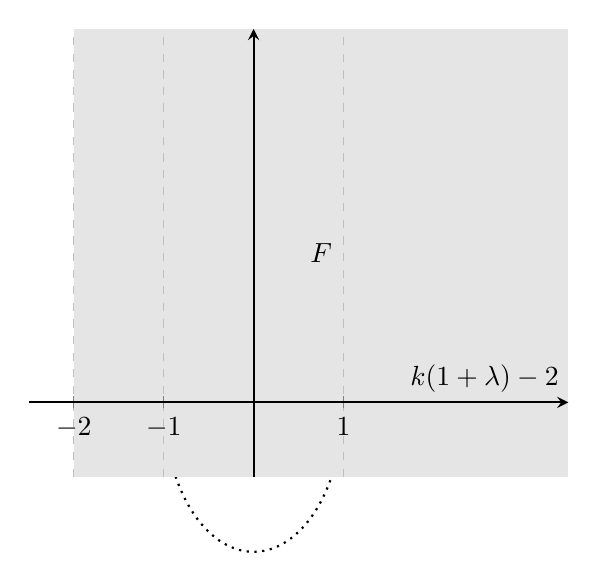
\begin{tikzpicture}
    \begin{axis}[
        axis lines = middle,
        axis line style = thick,
        xlabel = {$k(1+\lambda)-2$},
        ylabel = {},
        xmin=-2.5, xmax=3.5,
        ymin=-0.5, ymax=2.5,
        xtick={-2,-1,0,1},
        ytick=\empty,
        enlargelimits=false,
        clip=false,
        axis on top,
        grid = major,
        grid style=dashed,
        domain=-2:2,
        samples=100,
        no markers,
        every axis plot/.append style={thick},
        ]
        \addplot [black] {sqrt(1-x^2)}; % Upper semicircle
        \addplot [dotted] {-sqrt(1-x^2)}; % Lower semicircle
        \node at (axis cs: 0, 1) {\textbullet};
        \node at (axis cs: 0, 1) [above right] {$\mathbf{i}$};
        \filldraw[fill=gray!20, draw=none] (axis cs:-2, -0.5) rectangle (axis cs:3.5, 2.5) node[midway] {$F$};
    \end{axis}
\end{tikzpicture}
\end{document}